\chapter{Experimentální část}
Experimentální studii suspendace v mechanicky míchané nádobě provedla Bc.\,Zuzana Pavlíková v rámci své bakalářské práce na Ústavu chemického inženýrství VŠCHT Praha v roce 2011.

\section{Popis experimentu}
Náplní experimentu bylo měření průběhu homogenizace kapaliny v přítomnosti pevné fáze a následném zjišťování doby homogenizace. K provedení experimentu byla využita válcová nádoba z plexiskla o vnitřním průměru $T=\SI{0.29}{\meter}$ s plochým dnem, jenž byla opatřena čtyřmi radiálními narážkami o šířce $b=T/10$. Výška plnění nádoby byla zvolena $H=T$. 

\begin{figure}[h!]
\begin{center}
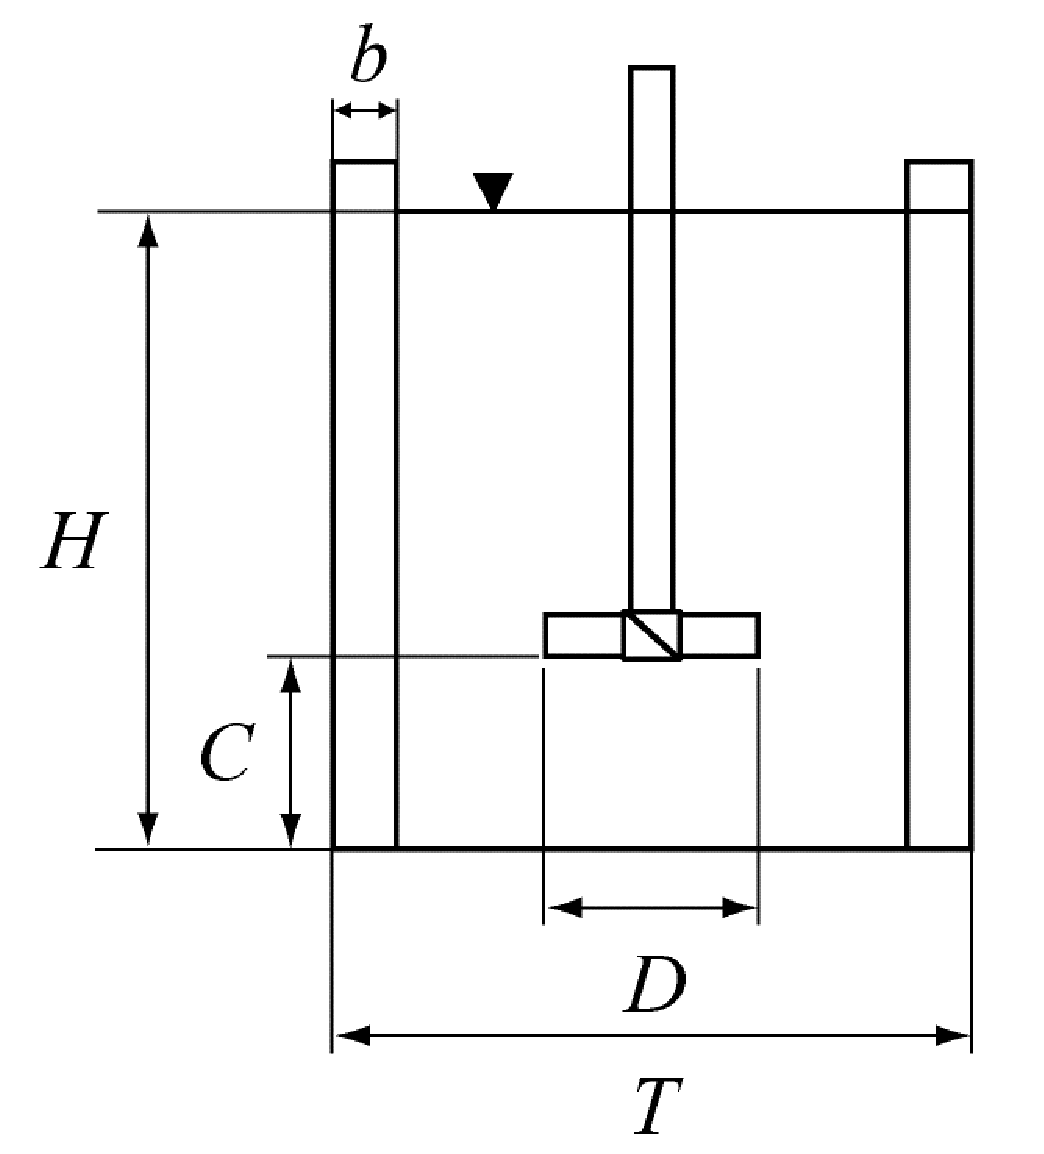
\includegraphics[scale=0.45]{images/mujedit.eps}
\caption{Geometrie experimentu}
\label{fig:nadoba}
\end{center}
\end{figure} 

Do nádoby $C=T/3$ ode dna bylo umístěno šestilopatkové míchadlo se šikmo skloněnými lopatkami (úhel zkosení \SI{45}{\degree}). Rychlost otáčení byla postupně volena  \SIlist[list-units = single]{3;4;5;6;7;8;9}{\per\second}. Celkový průměr míchadla činil $D=T/3$ a ostatní jeho rozměry jsou zobrazuje obr. XX.      

Jako vsádka byla použita voda a polyvinylpyrrolidon (PVP). Pevnou fázi tvořily červené kuličky z polyvinylchloridu (PVC) o průměru \SI{1.02}{\milli\meter}. Vsádka postupně obsahovala 5, 10 a 15 těchto kuliček. Vlastnosti kapalné a pevné fáze jsou shrnuty v 
